\hypertarget{four-places-of-prayer-haram}{%
  \chapter{Four places of prayer in Masjid al-Ḥarām}\label{four-places-of-prayer-haram}}

\chaptermark{Four places of prayer in Masjid al-Ḥarām}

The following is an excerpt (pp.\ 109–10) from \textit{The Story of a Pilgrimage to Hijaz} (Calcutta: Thacker, Spink \& Co, 1909) by His Highness, the Nawab Sultan Jahan Begam, Ruler of Bhopal.\\
\hrule

\begin{figure}
  \begin{center}
    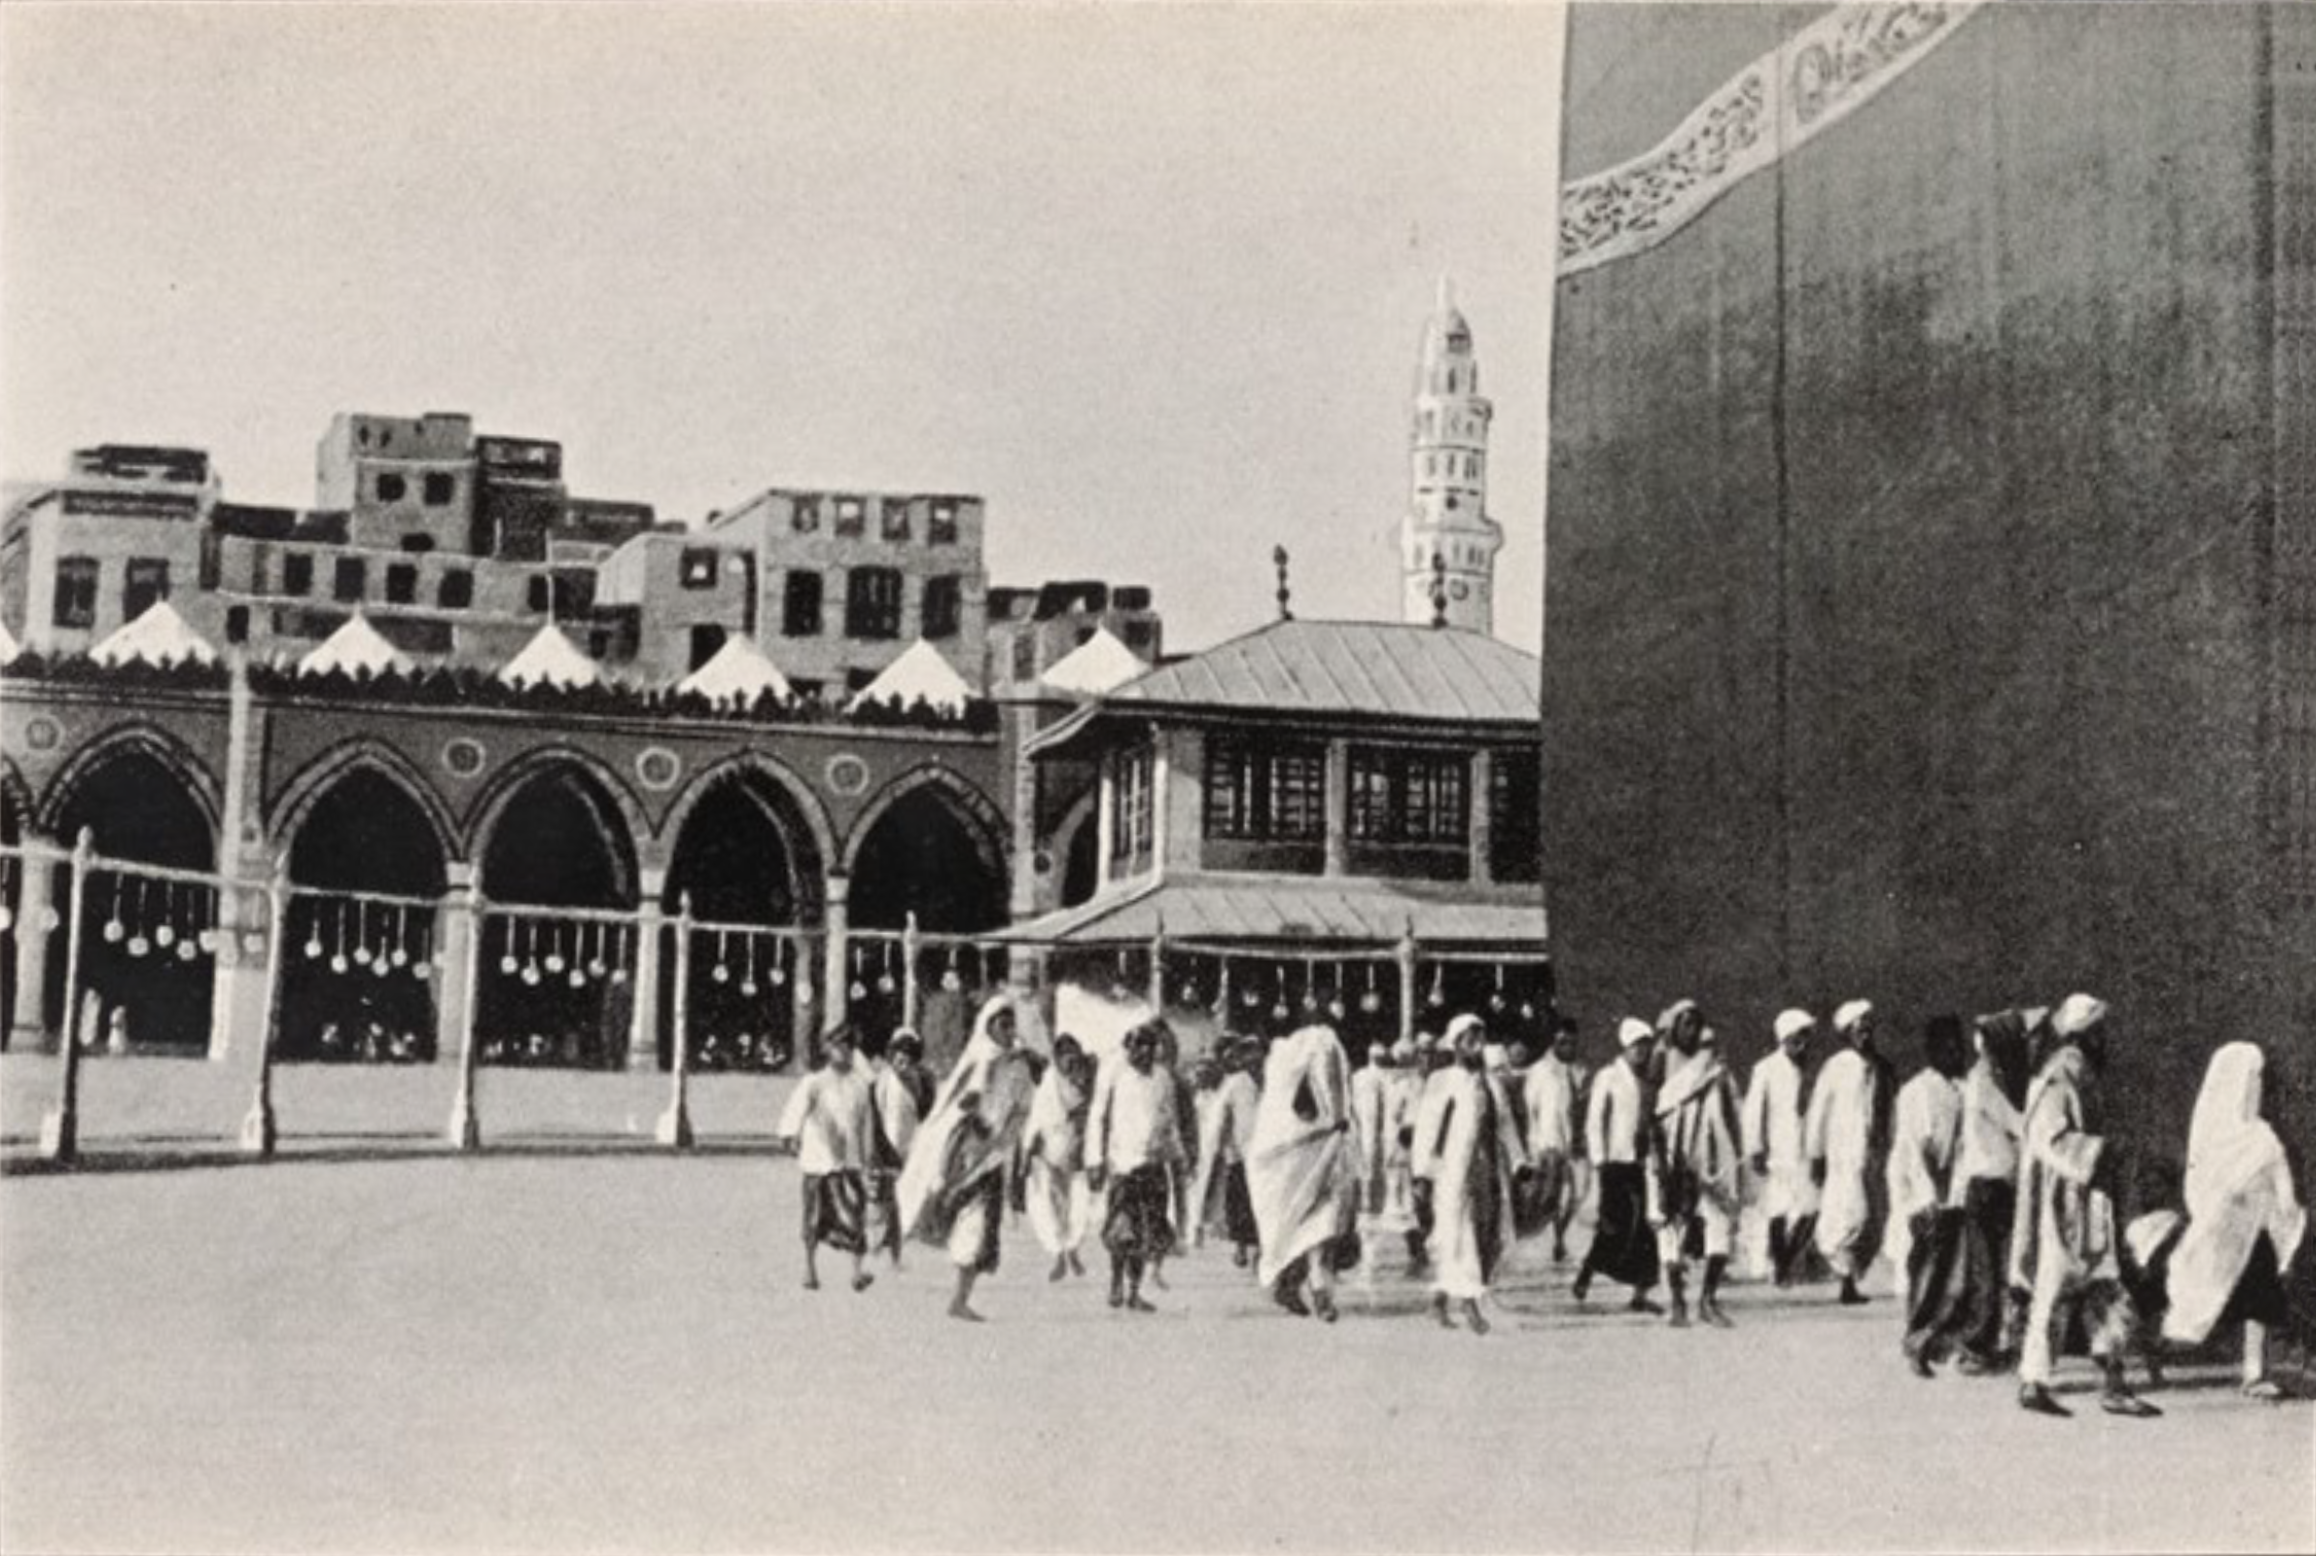
\includegraphics[width=0.84\textwidth]{images/haram2}
  \end{center}
  \caption*{Muṣallā Ḥanafī (p.\ 109).}
\end{figure}

\section*{Maqām Muṣallā Ḥanafī}

Inside the Ḥarām is a Muṣallā (place of prayer) surmounted by two brass spires where the Imam of the Ḥanafīs prays with those of his sect. The majority of the inhabitants of India and Turkistan are Ḥanafīs.

\section*{Maqām Muṣallā Shāfiʿī}

This Muṣallā, which stands close to the well of Zamzam, has a single brass spire. It is set apart for the worship of the Shāfiʿīs, the sect to which most Arabs belong.

\section*{Maqām Muṣallā Mālikī}

At this Muṣallā, which has one brass spire, the Imam of te Mālikīs stands to pray. The people of the Western countries are for the most parts[\textit{sic}] Mālikīs.

\section*{Maqām Muṣallā Ḥanbalī}

The Ḥanbalīs' Muṣallā has one brass spire. Most Arabs are followers of the Ḥanbalī school. The four Muṣallās above belong to the Sunnīs; The Shīʿas and the Khārijīs have no concern with them.

\begin{figure}[h]
  \begin{center}
    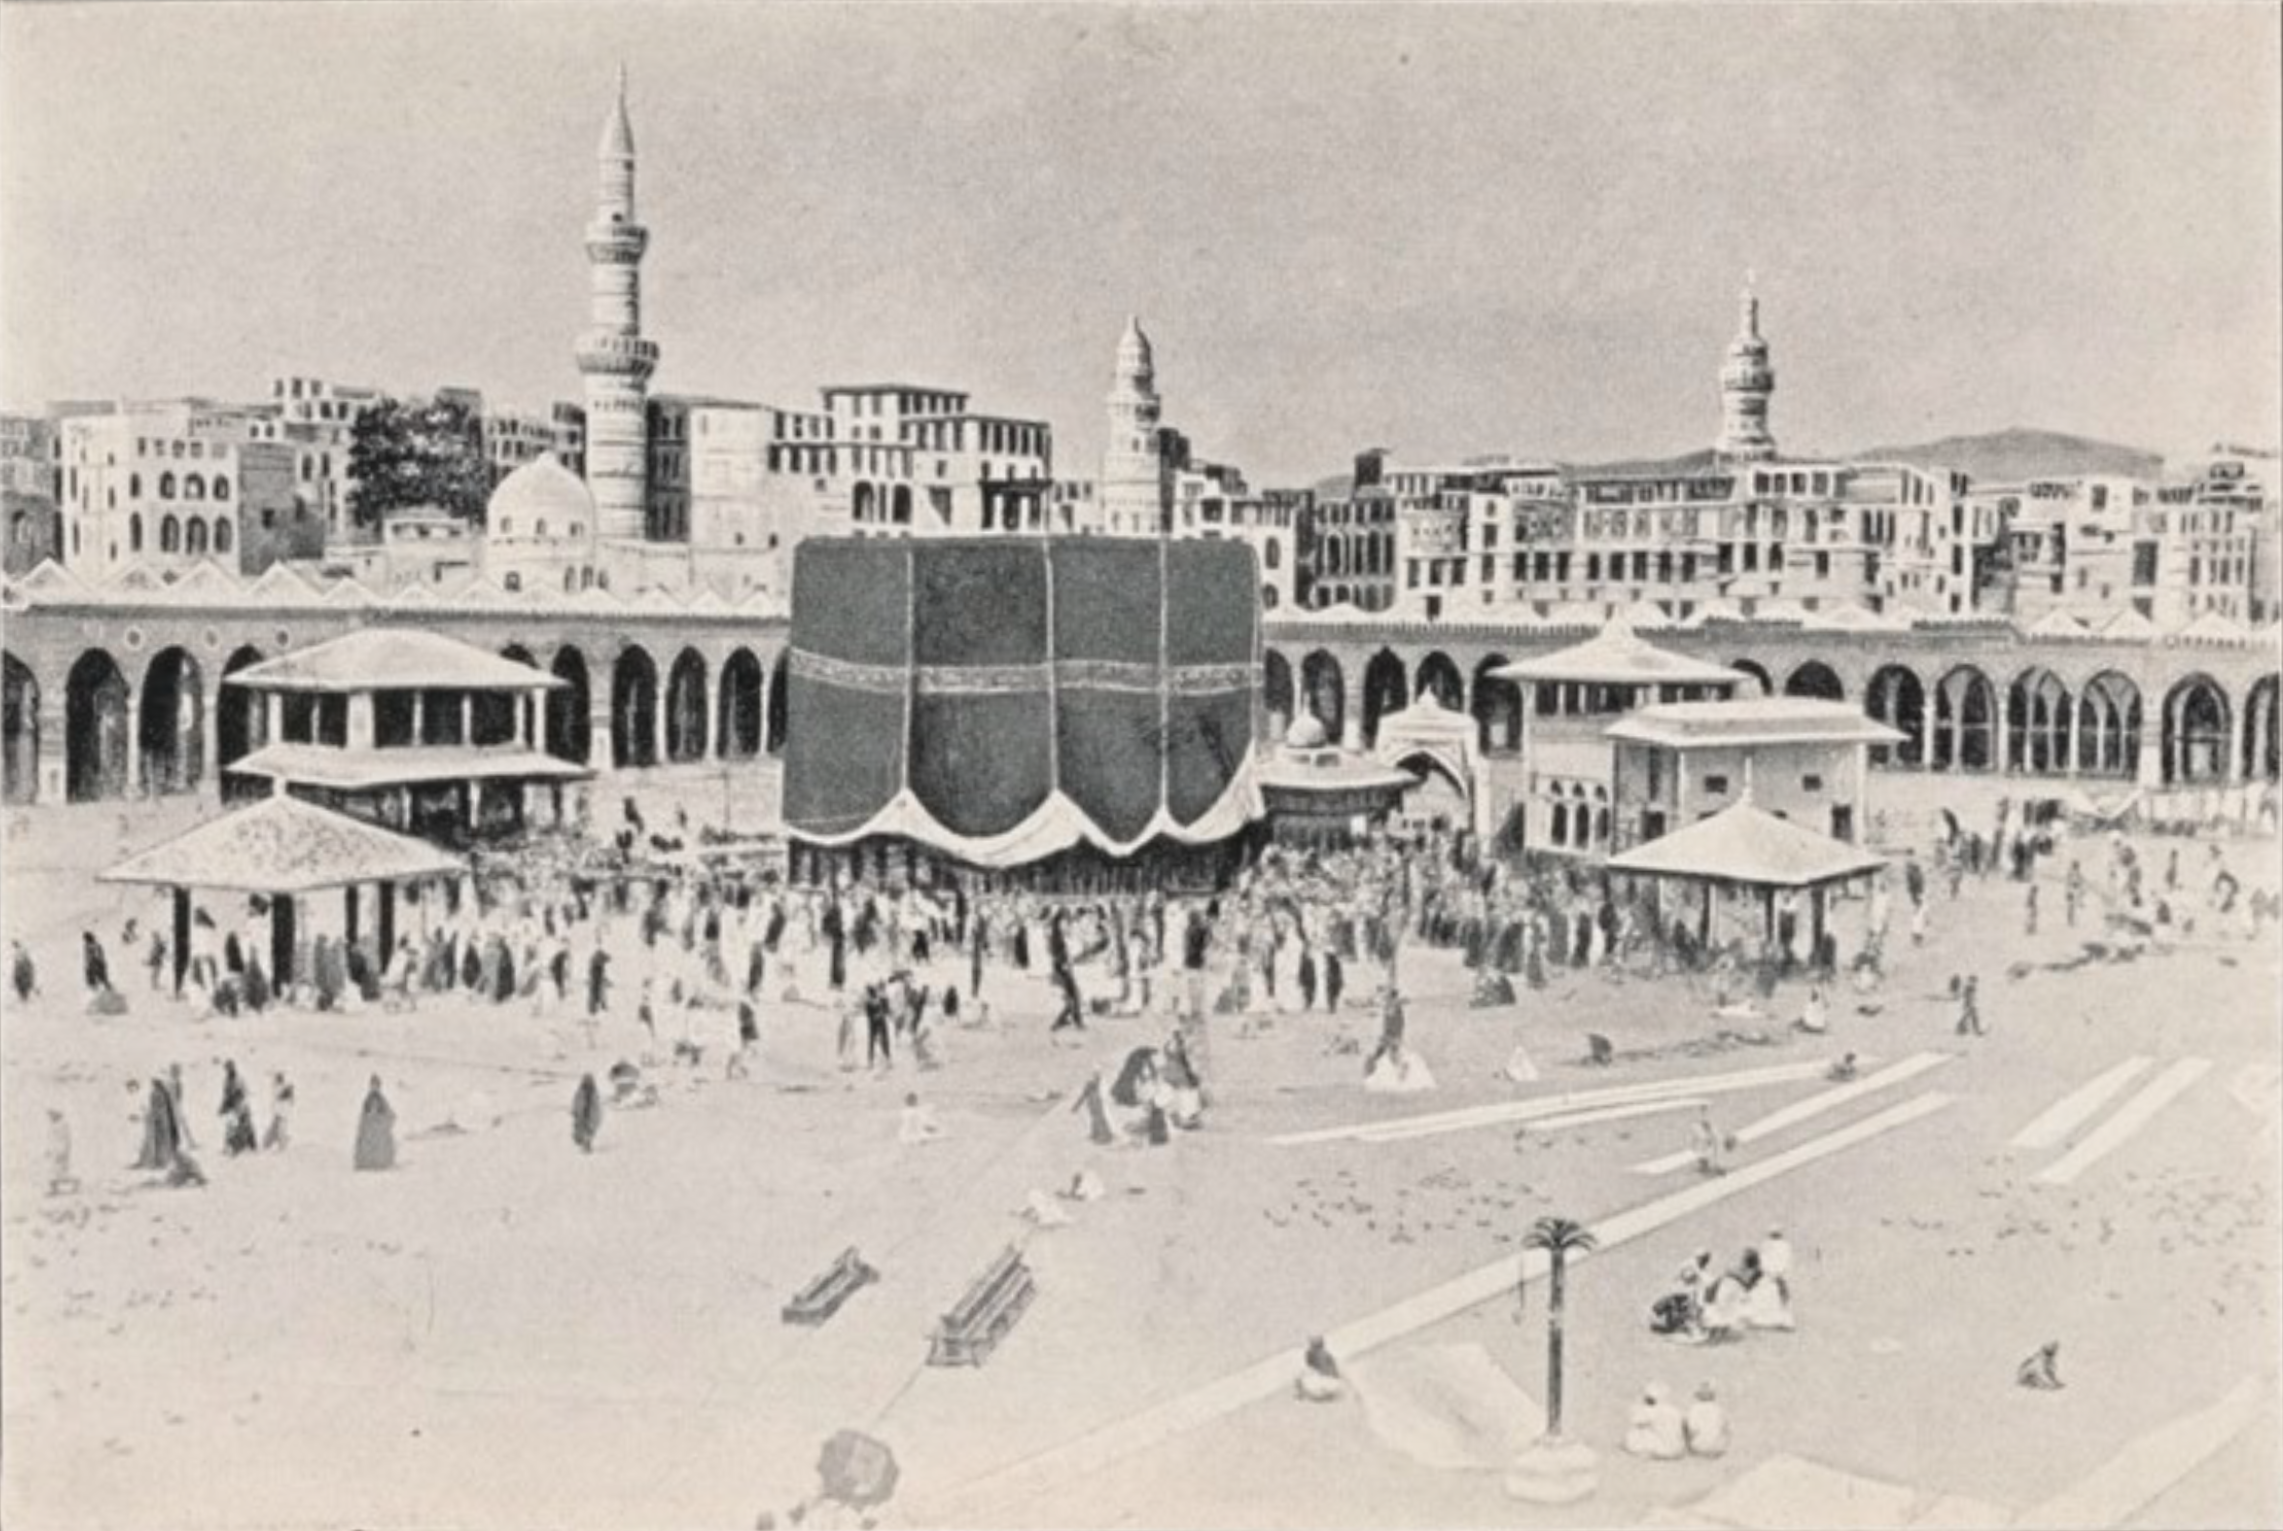
\includegraphics[width=0.84\textwidth]{images/haram1}
  \end{center}
  \caption*{Masjid al-Ḥarām al-Sharīf (p.\ 44).}
\end{figure}